\section{Circuiti RC e RL in corrente impulsata}
Per la prima parte dell'esperimento ci siamo posti come scopo quello di ricavare i valori del condensatore e dell'induttore, rispettivamente in un circuto RC ed in un circuito RL.

Prima di procedere abbiamo proceduto controllando la calibrazione delle sonde necessarie per misurare il segnale di tensione, attraverso l'uso dell'Oscilloscopio.

Per entrambe le configurazioni abbiamo utilizzato una resistenza di $R=10,1\Omega$. Tale scelta è stata motivata dal fatto che la resistenza dovesse essere molto inferiore a quella interna dell'Oscilloscopio di circa $1M\Omega$, per simulare nella realtà una resistenza infinita e, quindi, per non dividere i percorsi della corrente.

Per quanto riguarda la capacità abbiamo, invece, scelto un valore molto maggiore della capacità d'ingresso dell'Oscilloscopio di circa 20pF.

In entrambi i casi abbiamo montato il circuito come in figura, ponendo al posto di Z prima il condensatore e successivamente l'induttore.

\begin{figure} [H]
    \centering
    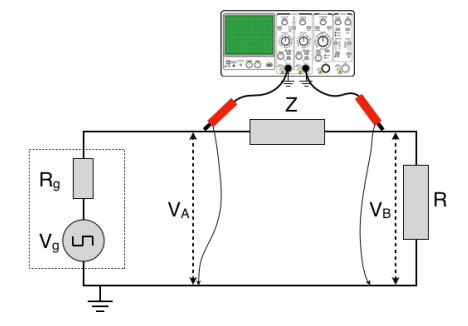
\includegraphics[scale=.9]{Immagini/Configurazione1.PNG}
    \label{fig:my_label}
    \caption{Configurazione circuiti RC e RL}
\end{figure}

\subsection{Configurazione circuito RC}
Dopo aver sistemato le componenti del circuito, abbiamo misurato il segnale di tensione ai capi di R e C mediante l'utilizzo di due sonde posizionate come nella figura sopra citata. Abbiamo, quindi, raccolto i dati servendoci di una chiavetta USB, scaricando dall'oscilloscopio i valori di tensione misurati con una frequenza di campionamento di $\frac{1\,\,\text{campionamento}}{0,001\,\,s}$.

Il fit dei dati è stato fatto linearizzando l'Eq. \ref{eq.8} ricavando quindi l'equazione di una retta. Il fit ed il calcolo dei parametri è esposto di seguito.
\begin{figure}[h!]
    \centering
    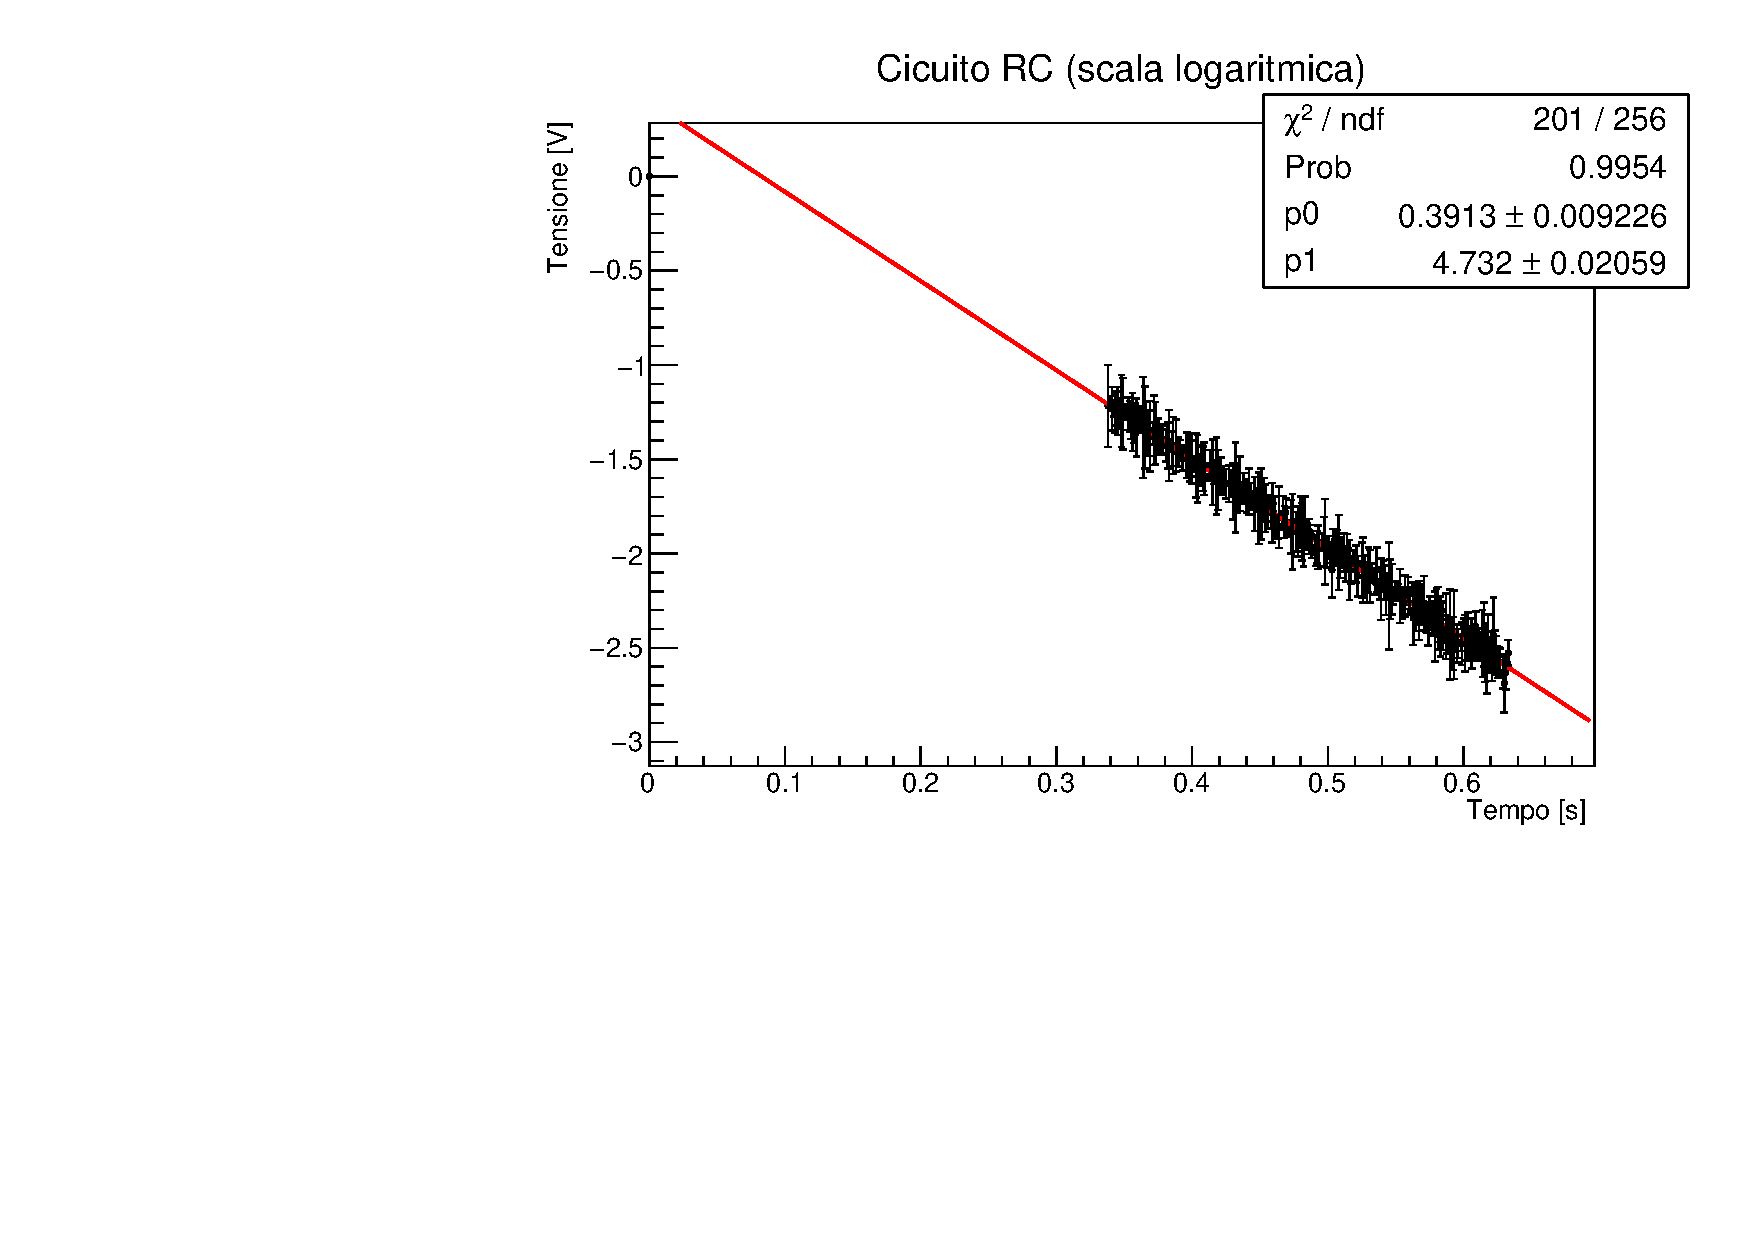
\includegraphics[scale=.4]{Immagini/CircuitoRC_logScale.pdf}
    \caption{La funzione che è stata usata per effettuare il fit è: $y=A-Bt$. Il parametro \textit{A} è associato a \textit{p0}, mentre \textit{p1} rappresenta il parametro \textit{B}}
    \label{fig: RC log scale}
\end{figure}
I parametri ricavati risultano quindi essere:
$$
V_0 = (1,479\,\pm\, 0,0136)\,V %l'errore l'ho ricavato come e^a \delta a
$$
$$
\tau = (0,211 \pm 0,001)\,s
$$

Il parametro che caratterizza il circuito è la costante di tempo $\tau=RC$. Nota R e ricavato il valore di $\tau$ dai dati presi con l'oscilloscopio, abbiamo, dunque, ricavato il valore della capacità del condensatore; essa risulta essere 
$$
C=\dfrac{\tau}{R} = (20,891\pm 0,229)\,mF
$$
l'errore è stato calcolato tramite la propagazione degli errori. 

\subsection{Configurazione circuito RL}

Dopo aver modificato le componenti del circuito, abbiamo misurato il segnale di tensione ai capi di R e L mediante l'utilizzo di due sonde posizionate come nella figura citata in precedenza. Anche in questo caso i dati sono stati raccolti direttamente dallo strumento con la stessa frequenza di campionamento utilizzata in precedenza.

In questo caso si è preferito non linearizzare la funzione con cui si sono interpolati i dati. Tale funzione è riportata nell'introduzione nell'Eq. \ref{eq. 7}. Riportiamo quindi di seguito i risultati e la discussione del fit.

\begin{figure}[H]
    \centering
    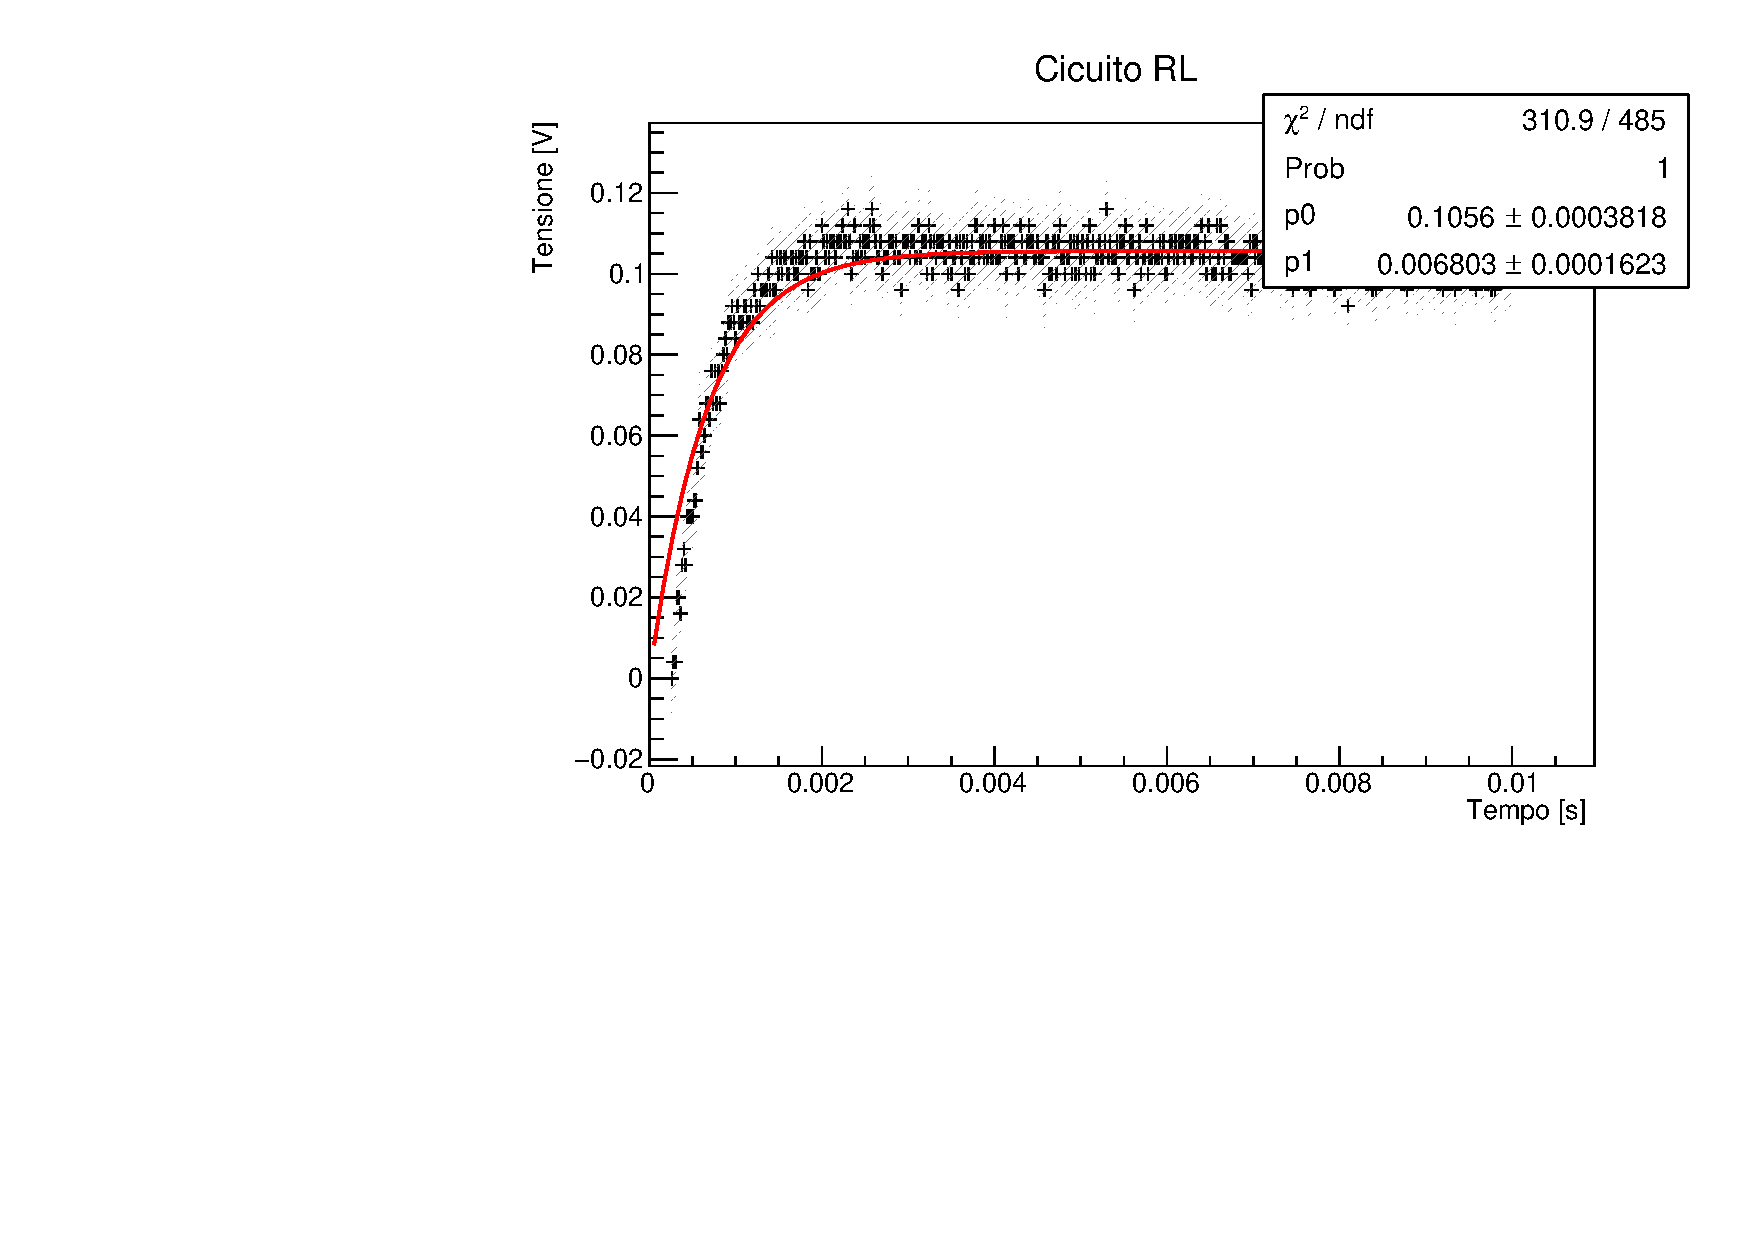
\includegraphics[scale=.4]{Immagini/CircuitoRL.pdf}
    \caption{}
    \label{fig:my_label}
\end{figure}

Il parametro che caratterizza il circuito è la costante di tempo $\tau=\frac{L}{R}$. Nota R e ricavato il valore di $\tau$ dai dati presi con l'oscilloscopio, abbiamo, dunque, ricavato il valore dell'induttanza; essa risulta essere pari
$$
\tau = (6,80\pm 0,16)\times 10^{-3}
$$
Da questo valore si ricava che l'induttanza risulta essere pari a 
$$
L= (68,68 \pm 1,753)\,mH
$$
